% !TeX root = ./00.ppgcc-2020.tex

\section{Implementações Preliminares}\label{sec:resultados}

No desenvolvimento desta pesquisa, uma vez determinado o modelo de operação
distribuída, com processamento nas bordas da rede, algumas experimentações e
algumas ferramentas de teste foram desenvolvidas. Aspectos desses
desenvolvimentos são descritos a seguir.
% obrigado hélio. % :-)

\subsection{Implementação com \python e \kafka}

\notaPA{Inserir Figura para auxiliar na compreensão, principalmente do problema encontrado.}
A primeira implementação e avaliação do \mfog realizada foi construída sobre a
linguagem \python com o sistema de fila de mensagens \kafka e a respectiva
biblioteca de conexão.
A escolha desse conjunto para a implementação ocorreu \hlhl{devido à ampla}
disponibilidade de bibliotecas de aprendizagem de máquina no ecossistema
\python e, à simplicidade geral da linguagem.
Na implementação desenvolvida, o sistema \kafka recebe mensagens e as armazena
em tópicos distribuídos em partições replicadas em nós de um \cluster,
gerenciados por um nó mestre e suportados pelo serviço de gerenciamento de
configuração distribuída \emph{Apache ZooKeeper}.
A aplicação \emph{Python} consome eventos através da interface \emph{Consumer API},
que expõe a distribuição através da associação de um consumidor às partições
mantidas pelo \kafka.

Para essa implementação, havia a hipótese de que a distribuição de
mensagens gerenciada pelo \kafka
se estenderia a processos consumidores, efetivamente distribuindo o volume de
mensagens entre eles igualmente.
Com esta hipótese, a arquitetura de comunicação seria formada por um elemento
produtor de descritores de fluxo (sensor do \nids) adicionando mensagens
ao tópico \kafka de entrada com $n$ partições, $n$ instâncias classificadoras
que consomem o tópico de entrada e produzem mensagens com os fluxos rotulados
para um tópico de saída, como ilustrado na Figura \ref{fig:python-kafka}.

\begin{figure}[htb]
    \centerline{
      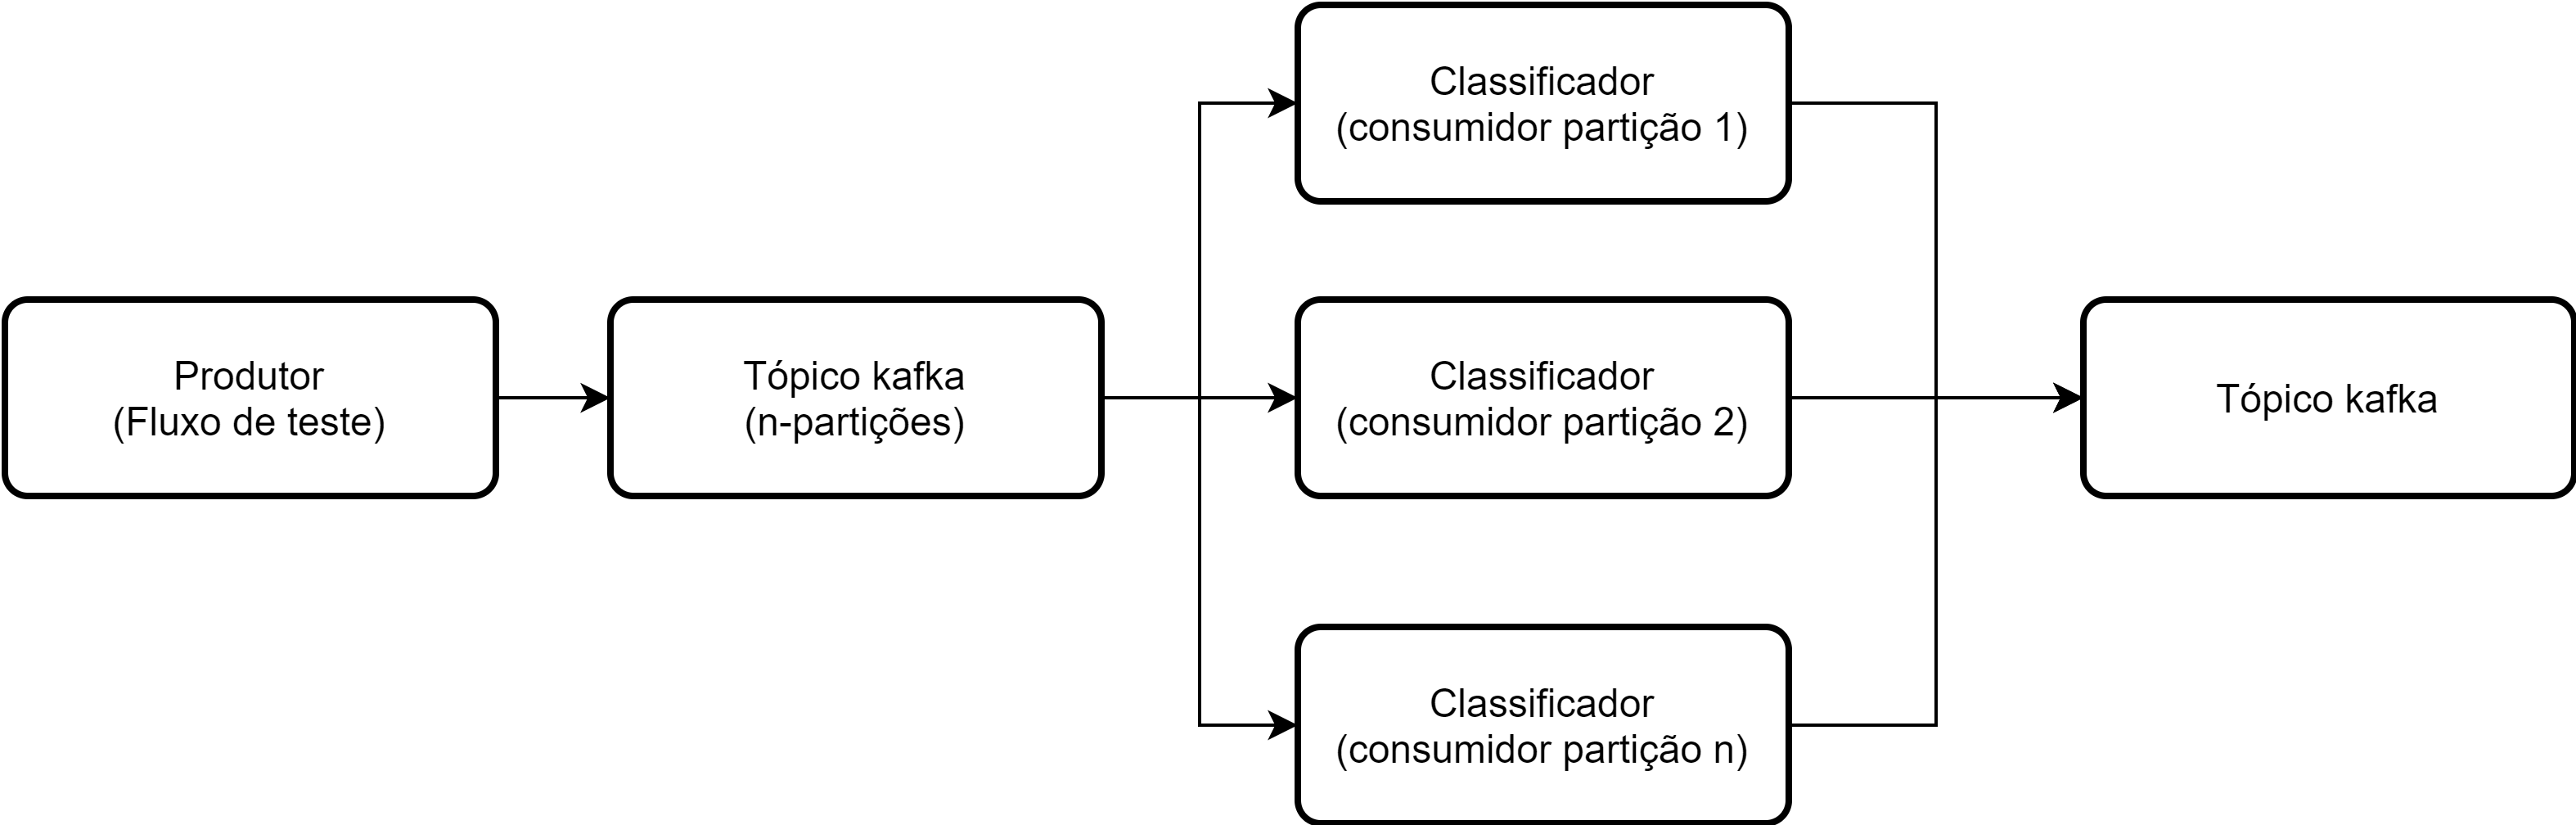
\includegraphics[width=\linewidth,page=1]{figures/python-kafka.png}
    }
    \caption{Hipótese de distribuição de carga com Apache Kafka e Python.}
    \label{fig:python-kafka}
\end{figure}

No entanto, a hipótese foi refutada nos experimentos realizados.
Os experimentos em questão\footnote{Código fonte disponível em
\url{https://github.com/luis-puhl/minas-py}.} foram compostos de 8 processos
consumidores e um processo produtor cujos programas foram escritos em Python com
a biblioteca \emph{confluent-kafka} versão $1.0.0$.
Além do programa, uma instância do par \kafka versão $2.2.0$ (git $121308c$) e
\emph{Apache ZooKeeper} com o tópico de entrada de 8 partições.
% A hipótese era que, como o número de partições igualava o número de consumidores,
% cada consumidor associaria-se a uma partição, distribuindo os dados igualmente
% entre os consumidores para a paralelização a execução.
A hipótese foi refutada quando observou-se que o número de
mensagens consumidas por um dos $8$ processos representava a maioria (mais de
$80\%$) do volume introduzido no sistema, o restante das mensagens sendo distribuído entre
outros $3$ processos e o restante dos processos não recebia nenhuma mensagem.
Portanto, a iniciativa de implementar o algoritmo MINAS em \python com \kafka e
atingir os objetivos de distribuição falhou, o que levou à reconsideração das
plataformas escolhidas.

% TODO: fiz a parte do "figura para auxiliar na compreensão" mas falta a parte
% do "principalmente do problema encontrado"

% TODO: Rodar o py-kafka-minas no i7, extrair contagem de exemplos por
% classificador, gerar gráfico de barras disso. (Faço???)
% UPDATE: Fiz isso no WSL FX-8300, não tive o mesmo resultado que tive em 2019.

% kafka_2.13-2.8.0, confluent-kafka==1.7.0
% ['load', [87344, 88918, 86770, 82051, 73662, 85475, 81423, 67814], 653457]
% [0, [], 85475]
% [1, [], 67814]
% [2, [], 81423]
% [3, [], 82051]
% [4, [], 88918]
% [5, [], 73662]
% [6, [], 87344]
% [7, [], 86770]
% loaded 653457 unloaded 653457
% 59.9 s ± 1.97 s per loop (mean ± std. dev. of 7 runs, 1 loop each)
% Author: Resultado excelente, porém:

% 2 years ago   (May 25th, 2019 12:34pm) 
% Adding kafka, 22 sec avg 0.045 item/s
% confluent-kafka==1.0.0
% kafka @ 121308c
% Local: Queue full 109983
% ['load', [13676, 13762, 13678, 13584, 13784, 13917, 13810, 13772], 109983]
% [0, [], 0]
% [1, [], 50181]
% [2, [], 0]
% [3, [], 0]
% [4, [], 0]
% [5, [], 0]
% [6, [], 0]
% [7, [], 0]
% loaded 109983 unloaded 50181
% Author: Resultado pior do que 2019, pois neste caso a lib usada pelo confluent-kafka
% gera um erro antes mesmo de carregar todos itens no kafka, a saída é pior ainda
% pois 1 consumidor de 8 pegam somente metade do total das mensagens.

\subsection{Implementação com \flink}

% \nota{citar ferramentas e a escolha só depois do python e kafka}
% \nota{entre flink e spark, outro grupo de pesquisa já está explorando spark}

A segunda alternativa explorada teve por inspiração o trabalho de
% \notaPA{Qual seria o outro grupo? Viegas et al. (2019)?}
% Author: Outro grupo é da UFMG acho. É pessoal mais próximo da Elaine, mas não
% o mesmo grupo de pesquisa exatamente.
% \citeonline{Viegas2019} e, \hlpa{como outro grupo de pesquisa} já estava explorando
\citeonline{Viegas2019} e, como outro grupo de pesquisa já estava explorando
o algoritmo na plataforma \emph{Apache Spark}, a segunda implementação
foi baseada na plataforma \flink.

A plataforma \flink tem modelos de processamento tanto de fluxos como em lotes.
O modelo em lotes é implementado como extensão do modelo de fluxos e, apesar de
não ser foco desse trabalho, mostrou-se útil para a construção da fase de
treinamento \emph{offline} do algoritmo \minas pois esta fase opera em lotes.
% , \hlpa{já que o conjunto consumido por
% esse módulo é limitado.}
% \notaPA{Não sei se compreendi corretamente. O modelo em lotes é pior, mas pode
% ser usado para treinamento offline por trabalhar com conjuntos de dados
% menores?}
% Author: O modelo em lotes não é pior, é uma extensão do modelo de fluxos.
% Nenhuma relação com o tamanho do conjunto.

% Um desafio encontrado durante o desenvolvimento da implementação do \mfog foi a falta
% de bibliotecas na plataforma \flink que disponibilizem versões adaptadas
% à plataforma de algoritmos base para o algoritmo MINAS.
% Em especial, a ausência dos algoritmos \emph{K-means} e \emph{CluStream}
% gerou carga imprevista sobre o processo de desenvolvimento
% resultando no atraso do processo de desenvolvimento.

% Esta implementação segue a arquitetura descrita na \refsec{descricao} e as
% avaliações e resultados esperados descritos neste \refcap{proposta}
% referem-se à implementação do \mfog na plataforma \flink.

Após desenvolvimento e testes em um computador pessoal, o sistema foi testado no
ambiente de testes como descrito na Seção \ref{sec:ambiente}, onde observou-se
que o uso de memória pela plataforma \flink excedia o disponível no sistema.
Com isso, optou-se por configurar dos parâmetros de memória do cluster
de maneira extrema, reduzindo os valores até que o cluster não conseguisse
iniciar e então retomando a configuração anterior, desta forma minimizando estes
valores.
Além disso, foi desativada a memória \emph{swap} para que o processo falhasse se
o uso de memória excedesse o recurso principal, deixando o sistema operacional e
o processo experimental mais responsivo.
Com estas configurações os resultados ficaram equivalentes à implementação de
referencia.
No entanto, apesar de exemplos de sucesso na literatura
\cite{lee2017data,Greco2019wearableStream,battulga2020fogguru}, o ambiente de
testes não permaneceu estável para execução de repetições do experimento,
necessitando reinicializações para que o controlador não ocupasse mais de $1GB$
na segunda execução, que é o limite dos recursos disponíveis.
% \notaPA{Definir "enorme"!}
% \hlpa{redução enorme} no desempenho que \hlpa{concluiu-se ser causada pelo uso excessivo de
% memória pela plataforma \flink}.
% \notaPA{Isso provocou uso de swap ou apenas mais acessos? Qual foi o gargalo?}
% Com a configuração dos parâmetros de memória do cluster, \hlpa{resultados
% \notaPA{Definir "resultados compatíveis com o esperado".}
% compatíveis com o esperado} foram obtidos; no entanto, apesar de exemplos de
% sucesso na literatura
% \cite{lee2017data,Greco2019wearableStream,battulga2020fogguru}, \hlpa{o ambiente de
% \notaPA{o código do Apache Flink é aberto?
% Esse problema não é apenas falta de liberação de memória?}
% testes não permaneceu estável para execução de repetições do experimento,
% necessitando reinicializações para que o controlador não ocupasse mais de $1GB$
% na segunda execução}, o que \hlpa{degradava imensamente} o desempenho.
% \notaPA{O termo "imensamente" é mesmo necessário?}

Em conclusão, apesar de promissora, a plataforma \flink ainda não suportava a
execução em dispositivos computacionais restritos de maneira confiável, sendo a
principal barreira o uso excessivo de memória, comum em plataformas do gênero
\emph{Big Data}.

% 2020-04-27T15:00:32.782 INFO  Classifier Ran baseline in 1408.8210000000001s
% jobmanager.heap.size: 100m
% taskmanager.memory.process.size: 800m
% taskmanager.memory.framework.heap.size: 64m
% taskmanager.memory.flink.size: 400m
% taskmanager.memory.managed.size: 100m
